% fig_island_rocof.tex
% TR-39: ROCOF vs power mismatch ΔP for IBR microgrid (H_eq=0.5s)
%
% df/dt = |ΔP| * f_nom / (2 * H_eq)
% NDZ: |ΔP| < 0.0200 pu
%
% Data points:
%  ΔP: -0.40 -0.30 -0.20 -0.10 -0.05  0.05  0.10  0.20  0.30  0.40
%  ROCOF: 20   15    10    5    2.5   2.5    5    10    15    20

\begin{tikzpicture}
\begin{axis}[
  name         = rocofax,
  width        = 0.80\textwidth,
  height       = 7.0cm,
  xlabel       = {Power mismatch $\Delta P$ [pu]},
  ylabel       = {ROCOF [Hz/s]},
  xlabel style = {font=\small},
  ylabel style = {font=\small},
  xmin=-0.48, xmax=0.48,
  ymin=0,     ymax=25,
  xtick        = {-0.4,-0.3,-0.2,-0.1,0,0.1,0.2,0.3,0.4},
  ytick        = {0,5,10,15,20,25},
  xticklabel style={font=\scriptsize},
  yticklabel style={font=\scriptsize},
  tick style   = {draw=none},
  axis line style={gray!50},
  grid         = major,
  grid style   = {gray!10, dashed},
  legend style = {at={(0.05,0.95)}, anchor=north west, font=\tiny,
                  draw=gray!60, fill=white},
  clip=false,
]

%% ROCOF curve (absolute value — symmetric about 0)
\addplot[blue!70!black, very thick, mark=*, mark size=2pt]
  coordinates {
    (-0.40, 20.00)
    (-0.30, 15.00)
    (-0.20, 10.00)
    (-0.10,  5.00)
    (-0.05,  2.50)
    ( 0.05,  2.50)
    ( 0.10,  5.00)
    ( 0.20, 10.00)
    ( 0.30, 15.00)
    ( 0.40, 20.00)
  };
\addlegendentry{ROCOF ($H_\mathrm{eq}=0.5$\,s)}

%% Detection threshold
\addplot[orange!70!black, very thick, dashed]
  coordinates {(-0.48, 1.0) (0.48, 1.0)};
\addlegendentry{ROCOF threshold $= 1$\,Hz/s}

%% NDZ shading: |ΔP| < 0.02
\addplot[red!20, fill=red!10]
  coordinates {(-0.020, 0) (-0.020, 25) (0.020, 25) (0.020, 0)}
  \closedcycle;
\addlegendentry{NDZ ($|\Delta P|<0.02$\,pu)}

%% NDZ boundary lines
\draw[red!60, dashed, thin]
  (axis cs:-0.020, 0) -- (axis cs:-0.020, 25);
\draw[red!60, dashed, thin]
  (axis cs:0.020, 0) -- (axis cs:0.020, 25);

%% Annotation
\node[blue!60!black, font=\tiny\bfseries, align=center]
  at (axis cs:0.30, 6)
  {$\mathrm{ROCOF} = \dfrac{|\Delta P|\cdot f_0}{2H_\mathrm{eq}}$};

\node[red!60!black, font=\tiny, align=center]
  at (axis cs:0.0, 22)
  {NDZ\\$\pm2\%$};

\end{axis}
\end{tikzpicture}
